\documentclass[12pt,a4paper,openany, oneside]{book}

\usepackage{fancyhdr}
 
\pagestyle{fancy}
\fancyhf{}
\lhead{\leftmark --- \rightmark}
\cfoot{\thepage}
\lfoot{Sebastian B. Hansen}
\rfoot{3r, N\o rre Gymnasium}


\usepackage{preamble}
\usepackage{referencekommandoer}
\usepackage{pdfpages}
\author{Sebastian Borgund Hansen \\ 3r, Nørre Gymnasium \\ SRP Fysik - Kemi}
\title{Infrarød-spektroskopi}
\date{\today}


\begin{document}
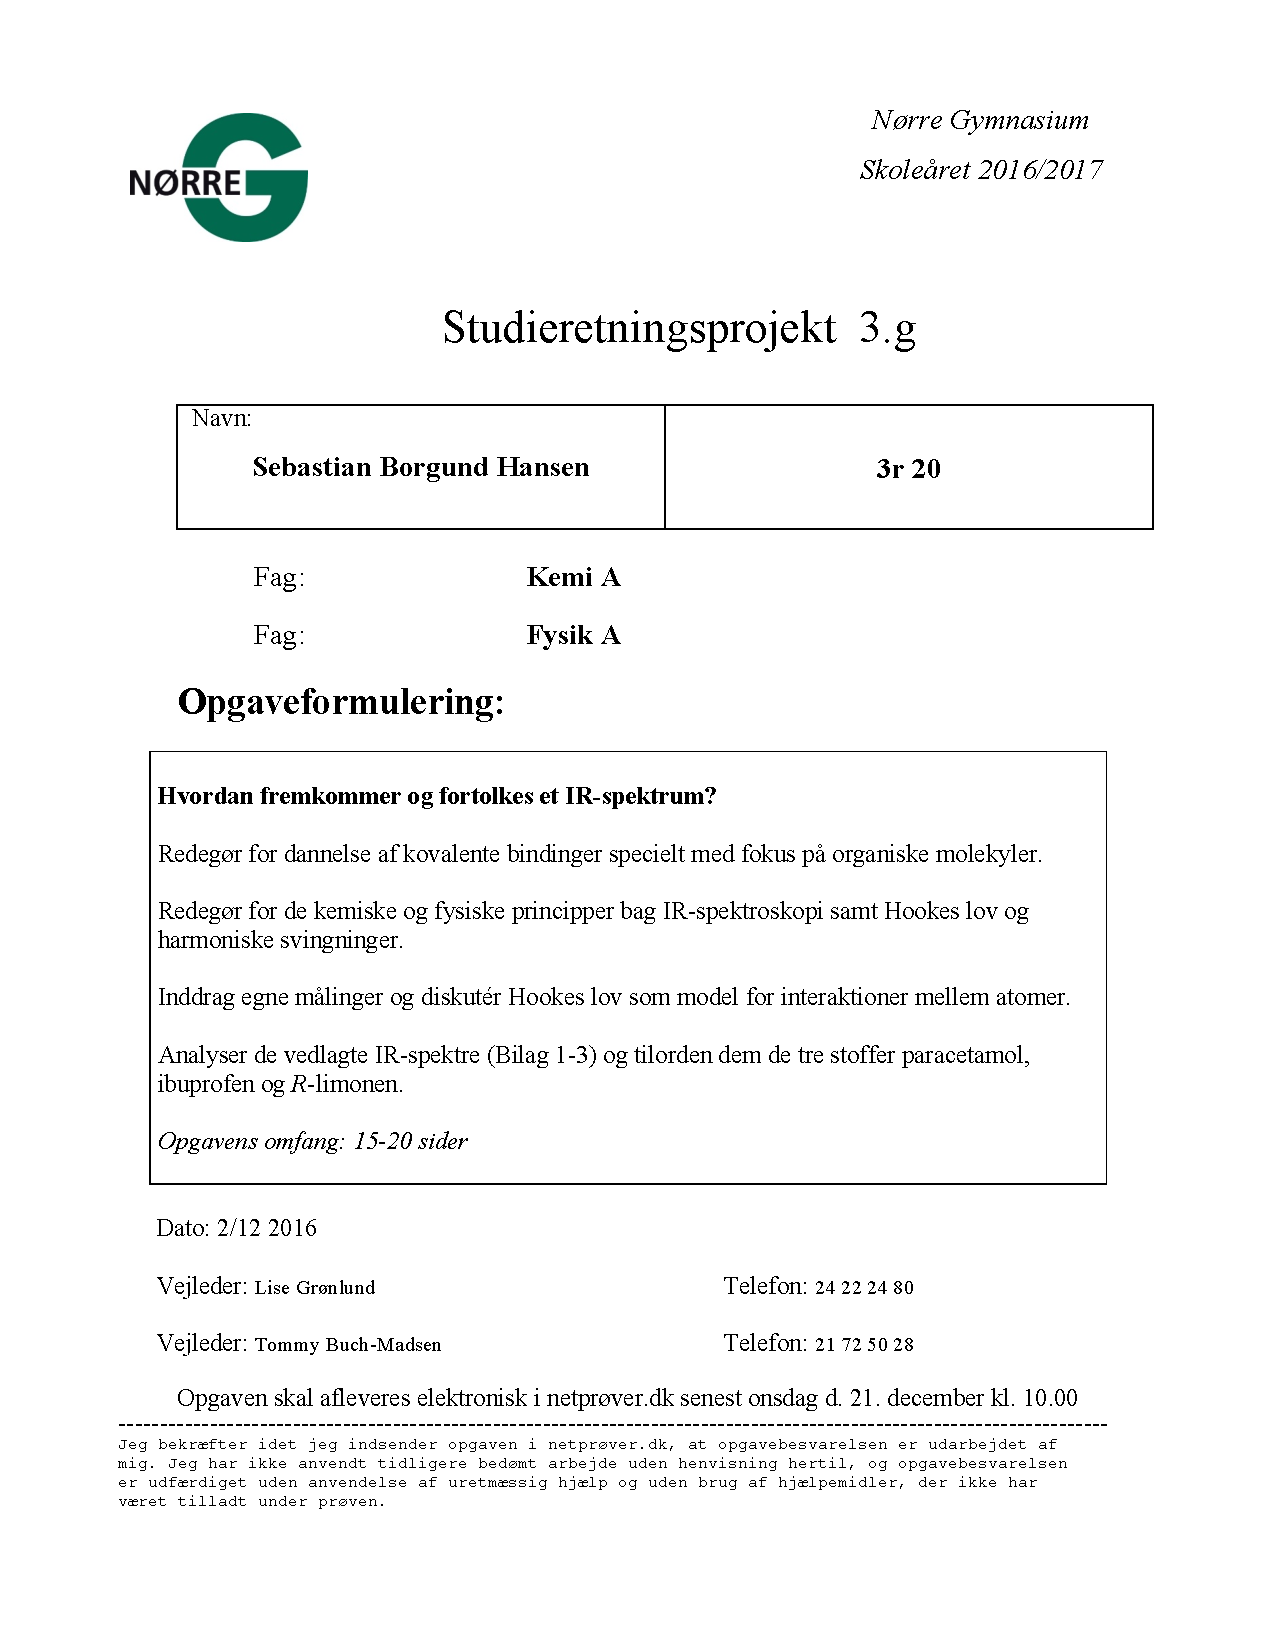
\includepdf[pages=1]{Forside.pdf}
\maketitle
\section*{Abstract}
This paper investigates the relationship between springs and the covalent bonds that form between atoms in molecules. Moreover the formation of covalent bonds in molecules is explained by looking at atomic and molecular orbitals. Furthermore the paper sheds light on infrared-spectroscopy as a tool to identification of chemical compounds. The paper includes a derivation of Hooke's law and the position function x(t] and the frequency of a harmonic oscillator. Four different experiments are made to conclude the following; 1. the validity of Hooke's law. 2. that a  mass attached to a spring performs a harmonic oscillating movement when displaced from its state of equilibrium. 3. that a system of 2 springs' stiffnesses, k, is equal to the sum of each spring's stiffness. 4. That a system of 3 springs' stiffness is equal to the sum of each of the springs stiffnesses. 
In the end of the paper the method of using infrared-spectroscopy as an identification tool is taken into use and three chemical compounds respectively - Paracetamol, Ibuprofen and R-limonen is linked to three different infrared spectrums. 

\tableofcontents


%KAPITEL 1
\chapter*{Indledning}
Infrarød-spektroskopi er et vigtigt værktøj indenfor kemien, da det i samfundet kan bruges til en bred vifte af ting. Her kan nævnes kvalitetskontrol af kemiske produkter, bestemmelse af alkoholprocent i blodet og til sikring mod gaslækager. 
\\

Denne opgave vil beskæftige sig med infrarød-spektroskopi som en metode brugt af kemikere til at identificere kemiske forbindelser. Den infrarøde-spektroskopi udnytter at bindinger mellem atomer i molekyler har en egenfrekvens som de vibrerer med. Disse vibrerende systemer kan i visse tilfælde betragtes som fjedre, som vi fra fysikkens side kender rigtigt godt til. Baggrunden for dannelsen af kovalente bindinger beskrives og ud fra Hookes lov, der i opgaven undersøges - både teoretisk og praktisk - sættes en formel, som skal kunne bestemme bølgetal, \={v}, for bestemte funktionelle grupper.


\chapter{Kovalente bindinger}
Mange kemiske forbindelser indeholder ikke ioner, men består i stedet af atomer, som er bundet tæt sammen i det vi kalder molekyler. De bånd, der holder atomerne sammen, formes når de omkredsende elektroner deles af de to kerner og skaber stabilitet. Et sådan bånd kaldes et kovalent bånd. I modsætning til ion-bindinger dannes kovalente bindinger når ingen af de to atomkerner, der indgår i bindingen har en stor nok elektronegativitet til at $rive$ elektronen væk fra det andet atom. Et af de simpleste eksempler på kovalent binding er i molekylet $H_2$. Kovalente bindinger er af stor betydning for den infrarøde-spektroskopi på grund af kovalente bindinger kan betragtes som fjedre.
\\
Vi vil se nærmere på dette i de følgende afsnit men vi vil indledningsvist lige snakke om atomernes elektronkonfiguration. 




\section{Elektroner}\label{elektroner}
Fra fysikkens verden ved vi følgende ting om elektroner. 

\begin{enumerate}
\item En elektrons position kan ikke bestemmes nøjagtigt. Det vi til gengæld kan sige noget om, er den orbital som elektronen befinder sig i. Vi kan bestemme størrelsen og formen på den orbital hvor der er en relativt stor chance for at finde den enkelte elektron i.

\item De orbitaler som elektronerne bevæger sig i karakteriseres ved kvantenumre $n = 1,2,3 ...$. Når n bliver større bliver afstanden til kernen større. Tilsvarende bliver energierne for orbitalerne også større med et større n. For n større end 1 kan der godt være forskellige orbitaler, som har samme værdi for n. En elektronskal indeholder orbitaler med samme værdi for n. Vi kan derfor vælge at benævne skallerne ved deres kvantenumre $1,2,3,4,5,6,7$ eller respektivt med bogstaverne $K,L,M,N,O,P,Q$. 

\item Orbitaler der har den samme værdi for n har nødvendigvis forskellige former. Se $2s$ og $2p$ orbitalerne, der behandles i afsnit \ref{sec:sp}

\item Da elektroner er fermioner har de en spin-værdi på enten $\frac{1}{2}$ eller $-\frac{1}{2}$ som respektivt er værdierne for spin-op og spin-ned elektroner, der tit og ofte skrives som små pile der vender opad eller nedad.
\\

\item Der kan maksimalt være 2 elektroner i hver orbital og de har hver deres spin.
\end{enumerate}

Det er desuden værd at notere sig, at der for atomer med mere end 2 elektroner gælder, at energien for elektronerne i orbitalerne at:

\bigskip
\begin{center}
$s$ elektroner $<$ $p$ elektroner $<$ $d$ elektroner $<$ $f$ elektroner
\end{center}
\bigskip

Da der kan være 2 elektroner i første skal, 8 i anden, 18 i tredje, 32 i den fjerde osv.. og atomer som udgangspunkt gerne vil have en så lav energi som muligt vil elektronerne starte med at fylde de orbitaler ud med lavest energiniveau først. Måden hvorpå elektronerne fylder orbitalerne ud er ved først at fylde en spin-op eller spin-ned elektron i orbitalen og dernæst det modsatte i orbitalen. Dette gør sig gældende for s-orbitalerne, men for de andre orbitaler, p, d og f orbitalerne, vil der først blive puttet en elektron i hver orbital før de fortsættes med at blive fyldt op. Dette leder os til orbitaler.
\section{Orbitaler}
For at opnå en dybere forståelse af hvorfor atomer vælger at gå sammen om at danne kovalente bindinger ser vi os nødsaget til lige at betragte et enkelt atoms elektronkonfiguration. De subatomare entiteter som elektroner er opfører sig ikke lige så pænt som Bohr formulerede i hans atommodel, hvor elektronerne bevæger sig i cirkulære baner, eller skaller, rundt omkring atomets kerne. Ifølge nyere teori har elektronerne en chance for at eksistere i visse områder omkring atomet som forklaret i forrige afsnit. Det laveste energiniveau en elektron kan befinde sig i, når det bevæger sig rundt om atomkernen er kugleformet og har tildelt navnet 1s orbitalen. Figur 1 er en skitse af 1s orbitalen plotteste i det kartesiske plan. 

\begin{figure}[ht!]
  \centering
  \begin{tikzpicture}[scale=2]
  \begin{scope}[font=\itshape]% to not type it every time, but better go for math mode


  \draw[-latex] (5,0)--(7,0) node[above]{x};
  \draw[-latex] (5,0)--(4.5,-0.7) node[above]{y};
  \draw[-latex] (5,0)--(5,1) node[above]{z};
  \orbital[color = purple, pos = {(5,0)}]{s} 
  \node[above] at (5.7,0.7) {1s orbital};

 		
  \end{scope}

  % correctly setting the background layer
  \begin{pgfonlayer}{backbackground}
  \fill[white](current bounding box.south west)rectangle
  (current bounding box.north east);
  \end{pgfonlayer}
  \end{tikzpicture}
  \caption{1s orbital} 
  \end{figure}
  
  I s-orbitalerne er der plads til netop 2 elektroner. At den første orbital hedder 1s henviser til at den tilhører skal 1. I 2. skal tilhører elektronerne 2s orbitalen. S på grund af orbitalerne som elektronerne forventes at være i har den samme form som 1s orbitalen og 2 fordi orbitalen knytter sig til den 2. skal. Orbitalen ligner 1s orbitalen til forveksling, men vil have en større radius da elektronerne der befinder sig i denne orbital har mere energi. Da vi ved, at der skal være 8 elektroner i den 2. skal for, at oktetreglen er opfyldt og atomerne derfor er stabile mangler vi stadigvæk at placere 6 elektroner. Disse elektroner vil befinde sig i de såkaldte p-orbitaler. Der eksisterer 3 forskellige p-orbitaler, som ligner sløjfer og som hver især indeholder 2 elektroner. De tre p-orbitaler benævnes respektivt $p_x$, $p_y$ og $p_z$, de er ortogonale på hinanden og ligger hhv. langs x-, y- og z-aksen. De er på figur 2 illustreret i et kartesisk koordinatsystem.
  
\begin{figure}[ht!]
  \centering
  \begin{tikzpicture}[scale=1.5]
  \begin{scope}[font=\itshape]% to not type it every time, but better go for math mode

 \draw[-latex] (0,0)--(1,0) node[above]{x};
  \draw[-latex] (0,0)--(-0.5,-0.7) node[above]{y};
  \draw[-latex] (0,0)--(0,1) node[above]{z};
  \orbital[pcolor = purple, pos = {(0,0)}]{py}
  \node[above] at (0.7,0.7) {p$_x$};
	
  \draw[-latex] (3,0)--(3.5,0.7);
  \draw[-latex] (3,0)--(4,0) node[above]{x};
  \draw[-latex] (3,0)--(2.5,-0.7) node[above]{y};
  \draw[-latex] (3,0)--(3,1) node[above]{z};
  \orbital[pcolor = purple, pos = {(3,0)}]{px} 
  \node[above] at (3.7,0.7) {p$_y$};

  \draw[-latex] (6,0)--(7,0) node[above]{x};
  \draw[-latex] (6,0)--(5.5,-0.7) node[above]{y};
  \draw[-latex] (6,0)--(6,1) node[above]{z};
  \orbital[pcolor = purple, pos = {(6,0)}]{pz}
  \node[above] at (6.7,0.7) {p$_z$};
  \end{scope}
  % correctly setting the background layer
  \begin{pgfonlayer}{backbackground}
  \fill[white](current bounding box.south west)rectangle
  (current bounding box.north east);
  \end{pgfonlayer}
  \end{tikzpicture}
  \caption{$2p_x$, $2p_y$, $2p_z$ orbital} \end{figure}

I 3 skal kan der være 18 elektroner. Disse elektroner bliver først fyldt ind i en 3s orbital, der ligner både 1s og 2s orbitalen i og med, at den er kugleformet. Radius på 3s orbitalen er større end på 2s orbitalen grundet det højere energiniveau. 6 af de resterende 16 elektroner kan dernæst findes i 3p orbitalerne. Der er, ligesom 2p-orbitalerne, også tre 3p-orbitaler - $3p_x$,$3p_y$ og en $3p_z$ orbital. For det illustrative formål kan vi bare betragte 2p-orbitalerne. 3p-orbitalerne ligner dem, men elektronerne kan bare befinde sig i større sløjfer end 2p-orbitalerne. 

Nu har vi kigget på de simpleste af orbitalerne, s- og p-orbitalerne. Der eksisterer også d og f orbitaler. f-orbitalerne vil jeg ikke beskæftige mig med, men p-orbitalerne er illustretet  figur 3. (Se figur 3 og 4) 
\\

\begin{figure}[ht!]
  \centering
  \begin{tikzpicture}[scale=1.5]
  \begin{scope}[font=\itshape]% to not type it every time, but better go for math mode

 \draw[-latex] (0,0)--(1,0) node[above]{x};
  \draw[-latex] (0,0)--(-0.5,-0.7) node[above]{y};
  \draw[-latex] (0,0)--(0,1) node[above]{z};
  \orbital[pcolor = purple, pos = {(0,0)}]{dxy}
  \node[above] at (0.7,0.7) {$d_{xy}$};
	
  \draw[-latex] (3,0)--(3.5,0.7);
  \draw[-latex] (3,0)--(4,0) node[above]{x};
  \draw[-latex] (3,0)--(2.5,-0.7) node[above]{y};
  \draw[-latex] (3,0)--(3,1) node[above]{z};
  \orbital[pcolor = purple, pos = {(3,0)}]{dxz} 
  \node[above] at (3.7,0.7) {$d_{xz}$};

  \draw[-latex] (6,0)--(7,0) node[above]{x};
  \draw[-latex] (6,0)--(5.5,-0.7) node[above]{y};
  \draw[-latex] (6,0)--(6,1) node[above]{z};
  \orbital[pcolor = purple, pos = {(6,0)}]{dyz}
  \node[above] at (6.7,0.7) {$d_{yz}$};
  
  \draw[-latex] (1,-2)--(2,-2) node[above]{x};
  \draw[-latex] (1,-2)--(0.5,-2.7) node[above]{y};
  \draw[-latex] (1,-2)--(1,-1) node[above]{z};
  \orbital[pcolor = purple, pos = {(1,-2)}]{dx2y2}
  \node[above] at (1.7,-1.3) {$x^{2}-y^{2}$};

  \draw[-latex] (5,-2)--(6,-2) node[above]{x};
  \draw[-latex] (5,-2)--(4.5,-2.7) node[above]{y};
  \draw[-latex] (5,-2)--(5,-1) node[above]{z};
  \orbital[pcolor = purple, pos = {(5,-2)}]{dz2}
  \node[above] at (5.7,-1.3) {$z^2$};
  
  \end{scope}
  % correctly setting the background layer
  \begin{pgfonlayer}{backbackground}
  \fill[white](current bounding box.south west)rectangle
  (current bounding box.north east);
  \end{pgfonlayer}
  \end{tikzpicture}
  \caption{$d_{xy}$, $d_{xz}$, $d_{yz}$, $x^{2}-y^{2}$, $z^2$ orbitalerne} 
  \end{figure}
\section{MO-teori og hybridisering}
I molekylær orbital teori ses der på fordelingen af elektroner i molekyler på samme måde som vi ser på fordelingen af elektroner i atomer.\refUniphys{186} Måden hvorpå vi bestemmer hvordan en elektron opfører sig på i et molekyle er ved hjælp af kvantemekanik og en bølgefunktion $\Psi$.\refUniKemi{149} På denne måde kan energien af en elektron og formen på det område hvori en elektron bevæger sig i bestemmes. Som vi i afsnit \ref{elektroner} fandt ud af, havde elektroner nogle områder hvori de havde den størst mulige change for at blive fundet i. Disse områder kaldte vi orbitaler. Ligesom atomer har orbitaler, har molekyler ligeledes også orbitaler hvori elektronerne har en stor chance for at blive fundet i. Forskellen på atomer og molekyler er, at elektroner i molekyler kan findes nær en hvilken som helst kerne i molekylet i stedet for den ene kerne, som orbitalen hører til for et atom.\refUniKemi{149} Dette er netop hvorfor vi kalder disse orbitaler for molekylære elektronorbitaler eller bare molekylære orbitaler. Ligesom atomare orbitaler er molekylære orbitaler også fyldt når de indeholder præcist 2 orbitaler med modsat spin. 
\\

\begin{wrapfigure}{r}{0.55\textwidth}
  \centering
  \begin{tikzpicture}[scale=1.5]
  \begin{scope}[font=\itshape]% 

  \draw[-latex] (0,-1)--(0,1) node[above]{Stigende energi};
  \orbital[color = purple, opacity = 1, scale = 2, pos = {(1,0.65)}]{s} 
  \orbital[color = purple, opacity = 1, scale = 2, pos = {(2,0.65)}]{s} 
  \node[above] at (1,0.5) {+};  
  \node[above] at (2,0.5) {+};
  \node[above] at (0.9,-0.15) {s orbital};
  \node[above] at (2.1,-0.15) {s orbital};
	\draw[-latex] (2.5,0.65)--(3.5,-0.10);
 		
 		
 		
 \orbital[color = purple, opacity = 0.2, scale = 2, pos = {(4,-0.5)}]{s} 
  \orbital[color = purple, opacity = 0.2, scale = 2, pos = {(4.5,-0.5)}]{s}  	
  	
  \node[above] at (4.2,-1.5) {Bindende orbital $\sigma_s$};
 	\node[above] at (4,-0.65) {+}; 
 	\node[above] at (4.5,-0.65) {+}; 
  \end{scope}

  \begin{pgfonlayer}{backbackground}
  \fill[white](current bounding box.south west)rectangle
  (current bounding box.north east);
  \end{pgfonlayer}
  \end{tikzpicture}
  \caption{Sigma-binding \label{fig:sigmabinding}}
   \end{wrapfigure}

Da vi så på de atomare orbitaler gav vi dem navnene, s, p, d og f. Molekylære orbitaler har også navne, men der vil i denne opgave ligge et fokus på $\pi$-orbitaler og $\sigma$-orbitaler. Lad os som eksempel betragte et eksempel på et homonukleært diatomisk molekyle som $H_2$. De to hydrogenatomer der er bundet sammen har hver især deres egen elektron, men når de er tilpas tæt nok på hinanden vil elektronerne i deres 1s orbitaler overlappe. Da elektronerne er negativt ladede og de 2 hydrogenkerner er positivt ladede, vil elektronerne blive tiltrukket af begge kerner og have et lavere niveau af energi ved, at befinde sig mellem de to atomer, end de ville have isolerede.\refUniKemi{151} Elektronerne vil altså søge at befinde sig mellem de to kerner og derved stabilisere molekylet. Denne slags orbitaler kaldes \textbf{bindende} orbitaler, da de som navnet antyder binder molekylet sammen. Da der stadigvæk kun er plads til 2  elektroner i en orbital, vil elektroner der ikke kan indgå i bindende orbitaler indgå i anti-bindende orbitaler. Disse orbitaler er med til at destabilisere molekyler og er en af grundene til at alle atomer ikke kan gå i forbindelse med hinanden. De anti-bindende orbitaler findes ved at tage to orbitaler der overlapper hinanden og fjerne deres overlap. Nu er orbitalen ikke mellem atomerne mere og vil derfor ikke stabilisere molekylet længere. På figur\ref{fig:sigmabinding} er det illustreret hvordan to atomare orbitaler går sammen om at danne en bindende $\sigma_s$ orbital. 
\\

Når to atomare orbitaler går sammen om at danne en ny orbital kalder vi det en hybridisering. En $\sigma$-binding er altså en hybridorbital.
\\

En $\sigma$-orbital er også det vi kender som en $\sigma$-binding eller én type kovalent binding. Kovalente bindinger er defineret som molekylære bindinger, der involverer en deling af elektroner mellem to atomer.\refUniKemi{151}
\\

På samme måde som med $\sigma$-orbitalerne dannes $\pi$-orbitalerne ved, at to atomer befinder sig tæt på hinanden og elektronerne kan få en lavere energi ved at befinde sig der hvor orbitalerne overlapper. Det græske bogstav $\pi$ refererer til p-orbitalerne. Dette er fordi $\pi$-orbitaler oftest ses dannet ud fra netop p-orbitaler, men det skal nævnes, at de også kan dannes ud fra d orbitaler. På figur \ref{fig:ethen} ses hvordan 2 p-orbitaler går sammen om at danne en $\pi$-bindinger. 
	
Nu har vi set på både $\sigma$-orbitaler / bindinger og $\pi$-orbitaler / bindinger - men hver for sig. Hvis de to orbitaler eksisterer sammentidigt i et molekyle har vi faktisk en dobbeltbinding. Dobbeltbindinger er netop lavet af en $\sigma$- og en $\pi$-binding. Illustreret som en tegning ville det se ud på følgende måde, se Figur \ref{fig:ethen}.

\begin{wrapfigure}{r}{0.5\textwidth}
\begin{center}
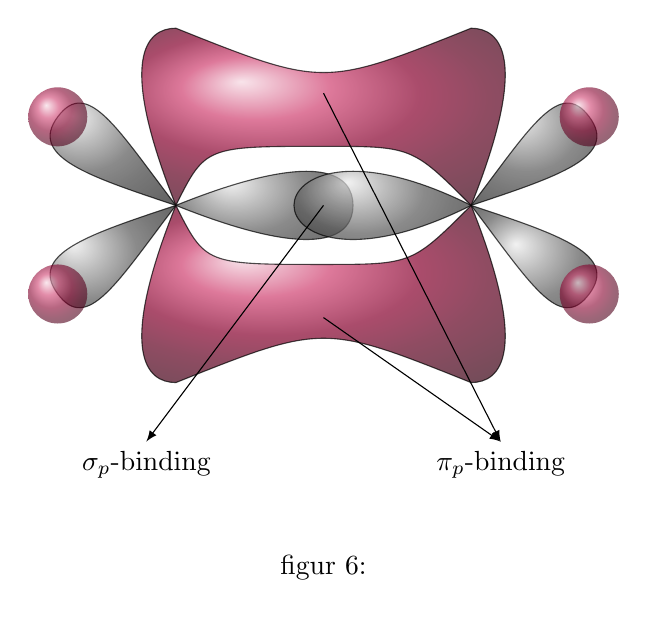
\begin{tikzpicture}[scale=0.75]

\shade[shading=ball, ball color=gray,draw,opacity=.7] (-2.5,0) .. controls (0,1) and     (.5,0.5) .. (.5,0)
.. controls (.5,-.5) and (0,-1) .. (-2.5,0);

\shade[shading=ball, ball color=gray,draw,opacity=.7] (2.5,0) .. controls (.5,1) and     (-.5,0.5) .. (-.5,0)
.. controls (-.5,-.5) and (.5,-1) .. (2.5,0);


\shade[shading=ball, ball color=gray,draw,opacity=.7] (-2.5,0) .. controls (-4,0.5) and     (-5,0.83) .. (-4.5,1.5)
.. controls (-4,2.17) and (-3.5,1.31) .. (-2.5,0);

\shade[shading=ball, ball color=gray,draw,opacity=.7] (-2.5,0) .. controls (-4,-0.5)     and (-5,-0.83) .. (-4.5,-1.5)
.. controls (-4,-2.17) and (-3.5,-1.31) .. (-2.5,0);


\shade[shading=ball, ball color=gray,draw,opacity=.7] (2.5,0) .. controls (4,0.5) and     (5,0.83) .. (4.5,1.5)
.. controls (4,2.17) and (3.5,1.31) .. (2.5,0);

\shade[shading=ball, ball color=gray,draw,opacity=.7] (2.5,0) .. controls (4,-0.5) and     (5,-0.83) .. (4.5,-1.5)
.. controls (4,-2.17) and (3.5,-1.31) .. (2.5,0);

\shade[shading=ball, ball color=purple,opacity=0.6] (4.5,1.5) circle (0.5);

\shade[shading=ball, ball color=purple,opacity=0.6] (4.5,-1.5) circle (.5);

\shade[shading=ball, ball color=purple,opacity=0.6] (-4.5,-1.5) circle (.5);

\shade[shading=ball, ball color=purple,opacity=0.6] (-4.5,1.5) circle (.5);


\shade[shading=ball, ball color=purple,draw,opacity=.7] (-2.5,0) .. controls (-3.5,2.5)     and (-3,3) .. (-2.5,3)
.. controls (0,2) .. (2.5,3)
.. controls (3,3) and (3.5,2.5) .. (2.5,0)
.. controls (1.5,1) .. (0,1)
.. controls (-2,1) .. (-2.5,0);


\shade[shading=ball, ball color=purple,draw,opacity=.7] (-2.5,0) .. controls (-3.5,-2.5)     and (-3,-3) .. (-2.5,-3)
.. controls (0,-2) .. (2.5,-3)
.. controls (3,-3) and (3.5,-2.5) .. (2.5,-0)
.. controls (1.5,-1) .. (0,-1)
.. controls (-2,-1) .. (-2.5,-0);

\draw[-latex] (0,0)--(-3,-4) node[below]{$\sigma_p$-binding};

\draw[-latex] (0,1.9)--(3,-4) node[below]{$\pi_p$-binding};

\draw[-latex] (0,-1.9)--(3,-4) node[below]{ };


\node[above] at (0,-6.5){figur 6: };
\end{tikzpicture}
\end{center}
\caption{Orbitaler i ethen \label{fig:ethen}}
\end{wrapfigure}

\textbf{note}: $\sigma$-bindingerne er stærkere end $\pi$-bindingerne da overlappet i sigmabindinger er større end i pibindinger.
\\

Det er ikke alle atomer, der har mulighed for at danne kovalente bindinger imellem sig. Når 2 atomer går sammen om at danne en kovalent binding er det fordi, at de hver især er ustabile. At de er ustabile er ens betydende med, at de ikke har deres orbitaler af højeste energiniveau fyldt ud. Når nogle atomer så alligevel ikke vælger at gå sammen og danne en kovalent binding er det oftest fordi, at de har for mange mange elektroner til, at de kun kan befinde sig mellem atomerne og danne en bindende $\sigma$-binding.
\\

Vi vil nu betragte nogle eksempler fra den organiske kemi.


\subsection{$\pi$- \& $\sigma$-orbitaler}

Da vi så de atomare orbitaler gav vi dem navnene, s,p,d og f. Molekylære orbitaler har også navne, men jeg vil i denne opgave primært have fokus på hhv. $\pi$-orbitaler og $\sigma$-orbitaler. Vi betragter et eksempel med et homonukleært diatomisk molekyle som $H_2$. De to hydrogenatomer der er bundet sammen har hver deres egen elektron, men når de er sig tilpas tæt nok på hinanden vil elektronerne mere eller mindre befinde sig mellem de to kerner. Da elektronerne er negativt ladede og de 2 hydrogenkerner er positivt ladede, vil elektronerne blive tiltrukket af begge kerner og have et lavere niveau af energi end de ville have isolerede (MANGLER NOTE GENERAL CHEMISTRY SIDE 150). Da elektronerne søger at have en så lav energi som muligt vil de befinde sig mellem de to kerner og stabilisere molekylet. Denne slags orbitaler kaldes \textbf{bindende} orbitaler, da de som navnet antyder binder molekylet sammen. På figur 4 er det illustreret hvordan to atomare orbitaler går sammen om at danne en bindende $\sigma_s$ orbital. 
\begin{center}
\begin{figure}[ht!]
  \centering
  \begin{tikzpicture}[scale=2]
  \begin{scope}[font=\itshape]% 

  \draw[-latex] (0,-1)--(0,1) node[above]{Stigende energi};
  \orbital[color = purple, opacity = 1, scale = 2, pos = {(1,0.65)}]{s} 
  \orbital[color = purple, opacity = 1, scale = 2, pos = {(2,0.65)}]{s} 
  \node[above] at (1,0.5) {+};  
  \node[above] at (2,0.5) {+};
  \node[above] at (1,0) {s orbital};
  \node[above] at (2,0) {s orbital};
	\draw[-latex] (2.5,0.65)--(3.5,-0.10);
 		
 		
 		
 \orbital[color = purple, opacity = 0.2, scale = 2, pos = {(4,-0.5)}]{s} 
  \orbital[color = purple, opacity = 0.3, scale = 2, pos = {(4.5,-0.5)}]{s}  	
  	
  \node[above] at (4.2,-1.5) {Bindende orbital $\sigma_s$};
 	\node[above] at (4,-0.65) {+}; 
 	\node[above] at (4.5,-0.65) {+}; 
  \end{scope}

  \begin{pgfonlayer}{backbackground}
  \fill[white](current bounding box.south west)rectangle
  (current bounding box.north east);
  \end{pgfonlayer}
  \end{tikzpicture}
  \caption{1s orbital} \end{figure}
	\end{center}
	
Denne bindende $\sigma$-orbital er faktisk det vi også kender som en $\sigma$-binding eller en kovalent binding. Kovalente bindinger er netop defineret som molekylære bindinger, der involverer at to atomer deler deres elektroner. 
\\

På samme måde som med $\sigma$-orbitalerne dannes $\pi$-orbitalerne ved, at to atomers befinder sig tæt på hinanden og elektronerne kan få en lavere energi ved at befinde sig i det sted hvor orbitalerne overlapper. $\pi$-orbitalerne adskiller sig alligevel fra $\sigma$-orbitalerne ved ikke at kunne blive dannet af overlap mellem s-orbitaler. En illustration af hvordan $\pi$-bindinger dannes ved et overlap af p-orbitaler: se figur 5. 
\begin{center}
\begin{figure}[ht!]
  \centering
  \begin{tikzpicture}[scale=2]
  \begin{scope}[font=\itshape]% 

  \draw[-latex] (-0.5,-1)--(-0.5,1) node[above]{Stigende energi};
  \orbital[pcolor = purple, opacity = 1, scale = 1, pos = {(1,0.65)}]{pz} 
  \orbital[pcolor = purple, opacity = 1, scale = 1, pos = {(2,0.65)}]{pz} 
  \node[above] at (0.8,-0.40) {$p_z-orbital$};
  \node[above] at (2.2,-0.40) {$p_z-orbital$};
	\draw[-latex] (2.5,0.65)--(3.5,-0.10);
  \node[above] at (1,0.5) {+};
  \node[above] at (2,0.5) {+};
 		
 \orbital[color = purple, opacity = 1, scale = 2, pos = {(4,-0.5)}]{s} 
  \orbital[color = purple, opacity = 1, scale = 2, pos = {(4.5,-0.5)}]{s}  	
  
 \orbital[color = lightgray, opacity = 0.3, scale = 2, pos = {(4,-1)}]{s} 
  \orbital[color = lightgray, opacity = 0.3, scale = 2, pos = {(4.5,-1)}]{s}  	  
  	
  \node[above] at (4.2,-2) {Bindende orbital $\pi_p$};
 		
 		
  \node[above] at (4,-0.90) {+};
  \node[above] at (4.5,-0.90) {+};		
 		
  \end{scope}

 \begin{pgfonlayer}{backbackground}
  \fill[white](current bounding box.south west)rectangle
  (current bounding box.north east);
  \end{pgfonlayer}
  \end{tikzpicture}
  \caption{ $\pi - binding$} \end{figure}
\end{center}
	
Nu har vi set på både $\sigma$-orbitaler /bindinger og $\pi$-orbitaler / bindinger - men hver for sig. Hvis de to orbitaler eksisterer sammentidigt i et molekyle har vi faktisk en dobbeltbinding. Dobbeltbindinger er netop en $\sigma$- og en $\pi$-binding. Illustret som en tegning ville det se ud på følgende måde, se Figur 6: 

\begin{center}
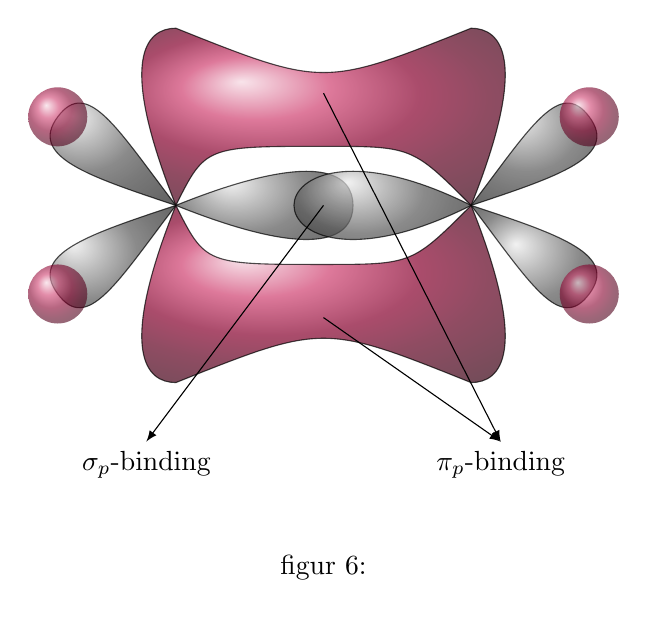
\begin{tikzpicture}[scale=0.75]

\shade[shading=ball, ball color=gray,draw,opacity=.7] (-2.5,0) .. controls (0,1) and     (.5,0.5) .. (.5,0)
.. controls (.5,-.5) and (0,-1) .. (-2.5,0);

\shade[shading=ball, ball color=gray,draw,opacity=.7] (2.5,0) .. controls (.5,1) and     (-.5,0.5) .. (-.5,0)
.. controls (-.5,-.5) and (.5,-1) .. (2.5,0);


\shade[shading=ball, ball color=gray,draw,opacity=.7] (-2.5,0) .. controls (-4,0.5) and     (-5,0.83) .. (-4.5,1.5)
.. controls (-4,2.17) and (-3.5,1.31) .. (-2.5,0);

\shade[shading=ball, ball color=gray,draw,opacity=.7] (-2.5,0) .. controls (-4,-0.5)     and (-5,-0.83) .. (-4.5,-1.5)
.. controls (-4,-2.17) and (-3.5,-1.31) .. (-2.5,0);


\shade[shading=ball, ball color=gray,draw,opacity=.7] (2.5,0) .. controls (4,0.5) and     (5,0.83) .. (4.5,1.5)
.. controls (4,2.17) and (3.5,1.31) .. (2.5,0);

\shade[shading=ball, ball color=gray,draw,opacity=.7] (2.5,0) .. controls (4,-0.5) and     (5,-0.83) .. (4.5,-1.5)
.. controls (4,-2.17) and (3.5,-1.31) .. (2.5,0);

\shade[shading=ball, ball color=purple,opacity=0.6] (4.5,1.5) circle (0.5);

\shade[shading=ball, ball color=purple,opacity=0.6] (4.5,-1.5) circle (.5);

\shade[shading=ball, ball color=purple,opacity=0.6] (-4.5,-1.5) circle (.5);

\shade[shading=ball, ball color=purple,opacity=0.6] (-4.5,1.5) circle (.5);


\shade[shading=ball, ball color=purple,draw,opacity=.7] (-2.5,0) .. controls (-3.5,2.5)     and (-3,3) .. (-2.5,3)
.. controls (0,2) .. (2.5,3)
.. controls (3,3) and (3.5,2.5) .. (2.5,0)
.. controls (1.5,1) .. (0,1)
.. controls (-2,1) .. (-2.5,0);


\shade[shading=ball, ball color=purple,draw,opacity=.7] (-2.5,0) .. controls (-3.5,-2.5)     and (-3,-3) .. (-2.5,-3)
.. controls (0,-2) .. (2.5,-3)
.. controls (3,-3) and (3.5,-2.5) .. (2.5,-0)
.. controls (1.5,-1) .. (0,-1)
.. controls (-2,-1) .. (-2.5,-0);

\draw[-latex] (0,0)--(-3,-4) node[below]{$\sigma_p$-binding};

\draw[-latex] (0,1.9)--(3,-4) node[below]{$\pi_p$-binding};

\draw[-latex] (0,-1.9)--(3,-4) node[below]{ };


\node[above] at (0,-6.5){figur 6: };
\end{tikzpicture}
\end{center}

$\sigma$-bindingerne er de stærkestee af de kovalente bindinger. Dernæst kommer $\pi$-bindingerne. blabla MO teori...


Det er nemmelig ikke alle atomer, der har mulighed for at danne kovalente bindinger imellem sig. Når 2 atomer går sammen om at danne en kovalent binding er det fordi, at de hver især er ustabile. At de er ustabile er ens betydende med, at de ikke har deres orbitaler af højeste energiniveau fyldt ud. Hver orbital vil gerne have en spin-op og en spin-ned elektron. Når nogle atomer så alligevel ikke vælger at gå sammen og danne en kovalent binding er det enten fordi, at de har for mange mange elektroner til, at de kun kan befinde sig mellem atomerne og danne en bindende $\sigma$-binding og derfor befinder sig i en orbital, der kræver et højere energiniveau og derfor er anti-bindende. 

\pagebreak
\section{Eksempler fra den organiske kemi}
Den organiske kemi er $carbonforbindelsernes$ $kemi$(Quote kemi A bog). Lad os indledningsvist se på methan, der har molekylformlen $CH_4$. Carbon skal kunne danne forbindelse til alle 4 hydrogenatomer, men hvis vi betragter carbons elektronkonfiguration vil vi lægge mærke til, at der kun er 2 ledige elektroner til at danne bindinger. Dette kan vi se ved at skrive de orbitaler op, som carbon fylder ud.
\\

Carbon har 6 elektroner og vil derfor først fylde 1s-orbitalen ud, dernæst 2s-orbitalen og til sidst vil der være 1 elektron i 2 af 2p-orbitalerne. Det er de 2 elektroner, der er alene i 2-orbitalerne der har mulighed for at danne en binding. Vi var dog interesserede i at danne 4 bindinger - netop til de 4 hydrogenatomer. Derfor exciteres ét af de elektroner, som befinder sig i 2s-orbitalen til en 2p-orbital sådan at der er 4 orbitaler med 1 elektron i hver. Denne excitering danner grundlag for en ny hybridorbital. Dette er $sp^3$-orbitalen. Navnet henviser til forholdet mellem s- og p-orbitaler. Der er 4 af disse. Hvis betragter carbons elektronkonfiguration nu vil vi se, at der først bliver fyldt op i $1s$-orbitalen og dernæst fyldes 1 elektron i hver af de fire $sp^3$-orbitaler. Dette giver anledning til at carbon nu kan danne 4 bindinger. Hver af de 4 $sp^3$-orbitaler går nu sammen med en $1s$-orbital som hydrogenatomerne har og danner en $\sigma$-binding således at molekylet stabiliseres. For at molekylet får en så lav energi som muligt vil bindingerne placere sig så langt væk fra hinanden som muligt og dette resulterer i at vi får den tetraidstruktur methan er kendt for at have (FODNOTE). 
\\

Et andet eksempel er ethen, hvis molekyl struktur er $C_{2}H_2$. Her har vi 2 carbonatomer der er bundet sammen af en dobbeltbinding. I dette eksempel skal hver carbonatom danne 4 bindinger - ét til hvert af de hydrogenatomer, der er bundet til carbonatomet og 2 til en $\sigma$- og en $\pi$-binding melem de 2 carbonatomer. Betragtes carbons elektronkonfiguration kan vi ligesom i det forrige eksempel se, at der kun er mulighed for at danne 2 bindinger. Derfor exciteres en elektron fra $2s$-orbitalen til en $2p$-orbital. Men da carbonatomet bliver nød til at behold en $2p$-orbital for at kunne danne en $\pi$-binding beholder den én af de 3 $2p-orbitaler$ der nu eksisterer. De 2 resterende $2p$-orbitaler går sammen med $2s$-orbitalen om at danne 3 $sp^{2}$-orbitaler. Således går 2 af de 3 $sp^2$-orbitaler til at danne $\sigma$-bindinger med de 2 hydrogenatomer og den sidste $sp^2$-orbital går sammen med det andet carbonatoms $sp^2$-orbital om at danne en $\sigma$-binding. Den $2p$-orbital, som ikke hybridiserede danner nu en $\pi$-binding der hvor der overlappes med det andet carbonatoms $2p$-orbital. 


\subsection{Kovalente bindinger}
Så det vi fandt ud af i dette afsnit var, at når 2 atomer går sammen og deler deres elektroner for at opnå en lavere energitilstand dannes nogle bindinger som vi kalder kovalente bindinger. Kovalente bindinger dannes når atomer, der har lige stor tilbøjelighed til at afgive elektroner mødes. Et eksempel på et organisk molekyle, der dannes kovalente bindinger er ethen. Her ses det tydeligt hvordan de to p-orbitaler går sammen i midten af molekylet om at lave en $\sigma_p$-(se figur 6). Vi fandt også ud af, i eksemplet med methan og ethen, at elektroner kan exciteres fra deres orbitaler for at danne nye hybridiserede orbitaler, som gør molekylet mere stabilt. Denne process kaldte vi hybridisering. Vi fandt også ud af at delte elektroner primært befandt sig mellem de positivt ladede atomkerner og den elektrostatiske tiltrækning mellem de to positivt ladede kerner og de to negativt ladede elektroner holder molekylet sammen samt at det bånd der blev dannet som et resultat af førnævnte er meget stærkt.

%KAPITEL 2
\chapter{IR-Spektroskopi}

\section{Fysikken bag}

\subsection{Arbejde og Hookes lov}
I den daglige omtale er arbejde et fysisk aktivitet der kræver energi. I fysikken bruger vi derimod arbejde som et udtryk for en kraft der virker på en genstand over en given distance. Arbejdet, A, som en genstand er blevet tilført på en strækning, s, med en kraft, F, er givet ved formlen
\\
\begin{center}
 $A=F \cdot s$. 
\end{center}
\bigskip

Dette er dog under antagelse af at kraften der virker på objektet er konstant samt at flytningen af objektet er i samme retning som kraften virker. 
Vi støder dog ind i problemer med at bestemme energien ud fra denne formel, hvis vi ser på et system hvor kraften bliver større jo længere væk fra startstedet, $s_0$, objektet bevæger sig. Formod nu, at vi ser på et objekt der bevæger sig langs en ret linje og hvor kraften bliver større jo længere vi flytter objektet. Da vil det samlede arbejde, $\sum A$ være lig summmen af alle de kræfter der har virket på objektet, siden størrelsen \textbf{arbejde} er en skalar.
\\
\begin{center}
$\sum A = A_1 + A_2 + ... + A_{n-1} + A_n$
\end{center}
\bigskip

For at bestemme denne størrelse deler vi den afstand, $s$, som objektet bevæger sig op i mindre dele $\Delta x_1$, $\Delta x_2$ osv. Vi deler disse afstande op i tilstrækkeligt små længder sådan at kraften der virker over de enkelte afstande er omtrent konstant. På denne måde kan vi beregne et totale arbejde som:
\\
\begin{center}
$A = F_1 \cdot \Delta x_1 + F_2 \cdot \Delta x_2 + ..$
\end{center}
\bigskip

Når vi får tilstrækkeligt mange længder og længderne samtidigt går mod at blive uendeligt små vil denne størrelse gå mod at blive integralet af F fra $x_1$ til $x_2$: 

\begin{center}
$A = \int\limits_{x_1}^{x_2} F dx$ 
\end{center}
\bigskip

Det er netop dette princip som Hookes lov benytter sig af. Hookes lov siger, at for en perfekt fjeder vil kraften direkte proportional til afstanden som fjederen er udtrukket. 

\begin{center}
$F = kx$
\end{center}
\bigskip

hvor k er stivheden er fjederen, F er kraften og x er den længden som fjederen er trukket ud. Med en perfekt fjeder skal der forstås at denne formel gælder uanset hvor langt man strækker fjederen ud eller presser den sammen. Dette er naturligvis en grov antagelse, men det er en god fysisk beskrivelse for at beregne størrelsen af en fjederkraft. Vi vil nu se på udledningen af denne sammenhæng.

Der vil her blive taget udgangspunkt i formlen 
\begin{equation}
V=\dfrac{1}{2} \cdot k \cdot (r-r_{0})^2
\end{equation}

Hvor V beskriver den potentielle energi en fjeder har når den er strukket en distance r ud fra hvilelængden $r_0$. 

\subsection{Udledning af Hookes lov}\label{Hookes}
Betragt den potentielle energi af en fjeder givet ved

\bigskip

\begin{equation}
V=\dfrac{1}{2} \cdot k \cdot (x-x_{0})^2
\end{equation}

\bigskip

Sæt nu $x_0 = 0$ og lad den initiale længde $x_i = x$ og den endelige udstrækningslængde $x_e = x + \Delta x$. Hvis vi ser på ændringen i den potentielle energi for systemet får vi da:

\bigskip

\begin{equation}
\Delta V = V_e - V_i = \dfrac{1}{2} \cdot k \cdot (x+ \Delta x)^2 - \dfrac{1}{2} \cdot k \cdot x^2
\end{equation}

\bigskip

Vi skriver $(x + \Delta x)^2$ ud og får:

\bigskip

\begin{equation}
\Delta V = V_e - V_i = \dfrac{1}{2} \cdot k \cdot (x^2 + 2x \Delta x + \Delta x^2) - \dfrac{1}{2} \cdot k \cdot x^2 
\end{equation}

\bigskip

I ligningen betragter vi nu de to størrelser $\dfrac{1}{2} \dot k \cdot x^2 og - \dfrac{1}{2} \cdot k \cdot x^2$. Disse to størrelser går ud med hinanden og efterlader os med

\bigskip

\begin{equation}
\Delta V = kx \Delta x + \dfrac{1}{2} \cdot k \cdot \Delta x^2
\end{equation}

Vi noterer os nu, at det første led på højresiden af lighedstegnet er lineært i $\Delta x$ og at det andet led på højresiden af lighedstegnet er kvadreret i $\Delta x$. $\Delta x$ er det vi betegner som en infinitesimal i kalkulus, hvilket betyder at størrelsen $\Delta x$ uendeligt lille. Når man så vælger at kvadrere noget der er så småt som $\Delta x$ vil størrelsen $\dfrac{1}{2} \cdot k \cdot \Delta x^2$ gå mod 0. Så vi ender med

\bigskip

\begin{equation}
\Delta V = kx \Delta x
\end{equation} 

\bigskip

Dette udtryk beskriver altså ændringen i den potentielle energi når vi udstrækker fjederen $\Delta x$, der er en uendelig lille udstrækning. 

\bigskip

Vi ser nu på ændringen af energi i et system, der er givet ved formlen 
\begin{equation}
\Delta E = \Delta E_{kin} + \Delta E_{pot}
\end{equation}

\bigskip

Ændringen i energi for et system er lig summen af ændringen i potentiel energi og kinetisk energi. 

Da dette er 0 for vores isolerede system får vi: 

\bigskip

\begin{equation}
\Delta E = \Delta E_{kin} + \Delta V = 0
\end{equation}

\bigskip

Hvilket, hvis størrelsen for den potentielle energi givet ved $\Delta V = kx \Delta x$ substitueres ind i stedet for $V$ i ligning  giver

\bigskip

\begin{equation}
\Delta E_{kin} + kx \Delta x = 0 \rightarrow \Delta E_{kin} = -kx \Delta x
\end{equation}

\bigskip

Nu vil vi bruge det fysiske resultat

\bigskip

\begin{equation}
\Delta E_{kin} = A = \textbf{F} \times \Delta \textbf{r} = F \cdot \Delta x (Arbejde-Energi teoremet)
\end{equation}

\bigskip

Notér at der i dette tilfælde regnes på en fjeder og der da kan ses bort fra at $F$ og $\Delta x$ vektorer. Dette kan vi tillade os da kraften virker i samme retning som fjederen trækkes. Vi tillader os da at regne arbejdet som $F \cdot \Delta x = A$.

Nu bruger vi resultatet 

\bigskip

\begin{equation}
\Delta E_{pot} = \textbf{F} \times \Delta \textbf{x} = F \cdot \Delta \textbf{x} = -kx \Delta x
\end{equation}

\bigskip

Ved division på begge sider af lighedstegnet af ligningen 

\bigskip

\begin{equation}
F \cdot \Delta x = -kx \Delta x
\end{equation}

\bigskip

Får vi det ønskede resultat: 

\bigskip

\begin{equation}
F = -k \cdot x
\end{equation}
\subsection{Harmoniske svingninger}\label{teori: Harmoniske svingninger}
En oscillerende bevægelse er en bevægelse hvor et objekt, som bliver flyttet fra sit hvilested og sluppet vil bevæge sig tilbage mod sit hvilested, hvor det vil bevæge sig forbi sit hvilested for igen at foretage gentagelser af netop dette for til slut at ende på sit hvilested igen. Dette kan eksempelvis ses hos penduler og masser bundet til fjedre.
\\

\begin{wrapfigure}{r}{0.4\textwidth}
\centering

\begin{tikzpicture}
\node[circle,fill=gray,inner sep=2.5mm] (a) at (0,0) {};
\node[circle,fill=gray,inner sep=2.5mm] (b) at (2,2) {};
\draw[decoration={aspect=0.3, segment length=3mm, amplitude=3mm,coil},decorate] (0,5) -- (a); 
\draw[decoration={aspect=0.3, segment length=1.5mm, amplitude=3mm,coil},decorate] (2,5) -- (b); 
\fill [pattern = north east lines] (-1,5) rectangle (3,5.2);
\draw[thick] (-1,5) -- (3,5);

\draw[-latex] (-1,2)--(-1,0) node[left]{$x$};

\end{tikzpicture}
\caption{Fjeder der trækkes i}
\label{figur fjeder}
\end{wrapfigure} 

Eksemplet der vil blive betragtet i dette kapitel er oscillerende bevægelse, der er hensigtsmæssig i forhold til at forstå IR-spektroskopier. Vi vil se på en masse der er bundet til en fjeder. se figur \ref{figur fjeder}.

Med udgangspunkt i figur \ref{figur fjeder} vil vi se på en masse der i den ene ende er fastgjort til noget stationært og i den anden ende er fastgjort til en kugle med en masse. Når kuglen ikke påvirkes af andre ydre kræfter en tyngdekraften vil kuglen opnå en hviletilstand hvor fjederkraften er lige så stor som tyngdekraften. Vi sætter denne hviletilstand til $x_0=0$. Når vi så begynder at påvirke system med en ydre kraft ved f.eks. at hive i kuglen vil fjederen svare tilbage ved at trække endnu hårdere i kuglen. Hvis vi op som den positive retning vil vi på figur \ref{figur fjeder} have flyttet kuglen en afstand $-x$ væk fra sin hvileposition vil fjederkraften givet ved Hookes lov, der blev beskrevet i \ref{Hookes} være givet ved $F_x=-k \cdot x$. Hvor F er fjedekraften, k er fjederkonstanten for den givne fjeder og x er afstanden flyttet fra hvilepositionen $x_0$
\subsection{Udledning af frekvens og positionsfunktion for harmonisk bevægelse}
Antag nu at Hookes lov gælder og at bevægelsen udelukkende foregår i y-aksens retning. Newton II giver da: 

\bigskip

\begin{center}
$F_x = -k \cdot x = m \cdot a_x = m \cdot x'' \rightarrow a_x = -\dfrac{k}{m} \cdot x$
\end{center}

\bigskip

Hvis massen, m, af objektet der er fæstnet til fjederen er konstant er størrelsen $\dfrac{k}{m}$ bare en konstant og da er $a_x \propto x$ til et hvert tidspunkt. Ud fra dette kan vi se at accelerationen er størst når x har opnået sin højeste positive værdi - kald denne størrelse $x_{max}$. Ydermere vil accelerationen være lig 0 når objektet passerer sit hvilepunkt, da x er lig 0 i netop dette punkt.
\\

Der bruges nu princippet om energibevarelse med den potentielle energi af systemet givet ved $V=\dfrac{1}{2} \cdot k \cdot x^2$ og den kinetiske energi af systemet givet ved $E_kin = \dfrac{1}{2} \cdot m \cdot v^2$.

\bigskip

\begin{center}
\begin{equation}
E_{system}=\dfrac{1}{2} \cdot m \cdot v^2 + \dfrac{1}{2} \cdot k \cdot x^2 = konstant
\end{equation}
\end{center}

Den totale energi $E_{system}$ er derfor  relateret til amplituden af $x_{max}$ sådan ,at når objektet når sin maksimale flytning $\pm x_{max}$, vil objektet stoppe og vende om. I dette punkt er hastigheden $v = 0$ og objektet har altså ikke nogen kinetisk energi. I dette punkt er $E_{system } = \dfrac{1}{2} \cdot k \cdot x^2$. Derfor må det gælde at

\bigskip
\begin{center}
\begin{equation}
E_{system}=\dfrac{1}{2} \cdot m \cdot v^2 + \dfrac{1}{2} \cdot k \cdot x^2 = \dfrac{1}{2} \cdot k \cdot (x_{max})^2
\end{equation}
\end{center}
\bigskip

eller 

\bigskip
\begin{center}
$\dfrac{1}{2} \cdot m \cdot v^2 + \dfrac{1}{2} \cdot k \cdot x^2 = \dfrac{1}{2} \cdot k \cdot (x_{max})^2 \rightarrow m \cdot v^2 = k \cdot (x_{max})^2 - k \cdot x^2 = k \cdot ((x_{max})^2 - x^2)$

$\rightarrow v^2 = \dfrac{k}{m} \cdot ((x_{max})^2 - x^2) \rightarrow v = \pm \sqrt[2]{\dfrac{k}{m}} \cdot \sqrt[2]{(x_{max})^2-x^2}$
\end{center}
\bigskip

\begin{wrapfigure}{r}{0.37\textwidth}
\begin{center}
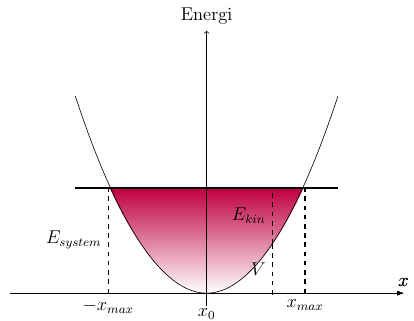
\includegraphics[scale=0.8]{Billeder/parabel}
\end{center}
\caption{Energi for fjedersystemet \label{fig:parabel}}
\end{wrapfigure} 

Med forbehold for fortegnet kan vi bruge denne relation til at bestemme hastigheden af objektet til en hver position x. Vigtigheden af det fundne udtryk $v = \pm \sqrt[2]{\dfrac{k}{m}} \cdot \sqrt[2]{(x_{max})^2-x^2}$ gør sig tydeligt på figur   \ref{fig:parabel} hvor energien er plottet op ad 2. aksen og udstrækningen fra hvilepositionen $x_0$ ad 1. aksen. Kurven repræsenterer den potentielle energi givet ved forskriften $V=\dfrac{1}{2} \cdot k \dot x^2$ og dette er en parabel. I højden $E_{system}$ er der en tyk sort streg, som repræsenterer den energibevarelse der er for systemet, da den skærer parablen i netop $-x_{max}$ og $x_{max}$ som er yderpositionerne for bevægelsen. Til en vilkårlig udstrækning, x, af fjederen kan vi bestemme den kinetiske energi som længden af den linje, der går fra den horisontale linje ned til parablen ved netop den x-værdi. Dér hvor den kinetiske energi er størst og altså farten er størst er ved hvilepositionen $x_0$. Det gælder altså at

\bigskip
\begin{center}
$\dfrac{1}{2} \cdot m \cdot (v_{max})^2 = E_{system}$ eller $v_{max} = \sqrt[2]{\dfrac{2 \cdot E_{system}}{m}}$
\end{center}
\bigskip

Men da det netop gjorde sig gældende at den maksimale potentielle og kinetiske energi begge er lig systemets energi $E_{system}$, og derfor også til hinanden, kan vi relatere $v_{max}$ til $x_{max}$.

\begin{center}
\begin{equation}
E_{system} = \dfrac{1}{2} \cdot k \cdot (x_{max})^2 = \dfrac{1}{2} \cdot m \cdot (v_{max})^2 \rightarrow v_{max} = \sqrt[2]{\dfrac{k}{m}} \cdot x_{max}
\end{equation}
\end{center}

Vi fandt udtrykket $v = \pm \sqrt[2]{\frac{k}{m}} \cdot \sqrt[2]{(x_{max})^2-x^2}$. Dette beskrev hastigheden til en udstrækning x. Vi ser os ikke tilfredse med en hastighedsfunktion alene. Vi vil også have stedsfunktionen. Denne findes ved at skrive den fundne ligning op som 

\begin{center}
\begin{equation}
\dfrac{dx}{dt} = v = \pm \sqrt[2]{\dfrac{k}{m}} \cdot \sqrt[2]{(x_{max})^2-x^2}
\end{equation}
\end{center}

Denne ligning integreres og løses for x ved hjælp af den matematiske metode \emph{seperation af de variable}, hvilket giver

\begin{center}
\begin{equation}
x = x_{max} \cdot sin(\sqrt[2]{\dfrac{k}{m}} \cdot t + C)
\end{equation}
\end{center}
\bigskip
Hvor C er en konstant. \emph{Notér} at sinus er en periodisk funktion og at positionen af x altså også er en periodisk funktion af tiden, som vi forventede. Perioden for bevægelsen, T, er den tid det tager for systemet at lave en oscilation. Da sinusfunktionen gentager sig selv hver eneste gang vi øger udtrykket inden i parantesen $sin(\sqrt[2]{\frac{k}{m}} \cdot t + C$ med $2 \pi$ må det altså gælde, hvis starttidspunktet t = 0, at en oscilation må tage

\begin{center}
\begin{equation}
\sqrt[2]{\dfrac{k}{m}} \cdot T = 2 \pi \rightarrow T = 2 \pi \sqrt[2]{\dfrac{m}{k}}
\end{equation}
\end{center}

Hvilket hvis $f = \dfrac{1}{T}$ giver

\begin{center}
\begin{equation}
f = \dfrac{1}{T} = \dfrac{1}{2 \pi} \cdot \sqrt[2]{\dfrac{k}{m}}
\end{equation}
\end{center}

Hvilket er et vigtigt resultat, som vi vil bruge til at bestemme bølgetal for funktionelle grupper i IR-spektroskopien. 
\section{Forsøg med Hooks lov}
I anledning af vigtigheden af Hookes' lov har jeg opstillet nogle forsøg. Forsøgene har dels til formål at eftervise validiteten af Hookes lov samt at anskueliggøre ideen om at kovalente bindinger kan betragtes som fjedre. Der er i alt 4 forsøg, det første skal vise at kraften som en fjeder trækker med når den bliver trukket i er direkte proportionelt med afstanden som fjederen bliver trukket ud og at proportionalitetsfaktoren er fjederkonstanten K. Det andet forsøg skal vise at stedfunktionen for et objekt der laver en oscillerende bevægelse kan skrives på formen $x(t) = A \cdot sin(B t + C) + D$, hvor A, B, C er konstanter. A bestemmes som amplituden på udslagene og B bestemmes som $B=\sqrt[2]{\dfrac{k}{m}}$. Det tredje forsøg skal vise, at hvis vi har et system af to fjedre, som er helt ens og vi hænger en masse i de to fjedre vil fjederkonstanten for systemet blive lig summen af de to fjedres fjederkonstanter. Det fjerde forsøg skal vise, at hvis vi har et system med flere forskellige fjedre og betragter dem som \textbf{én} samlet fjeder vil fjederkonstanten for systemet af fjedre være lig summen af de fjederkonstanter for fjedrene, som er med i systemet. Det fjerde forsøg er en generaliserende version af forsøg 3, da der indgår forskellige fjedrer. 

\subsection{Forsøg 1}
En luftpudebænk blev sat op og 2 kroge blev monteret. 1 for enden af luftpudebænken og en på en vogn. Der blev fastgjort en fjeder mellem de to kroge. Derefter blev der trukket i vognen og målt sammenhørende værdier mellem afstanden som vognen blev trukket ud og kraften målt på et newtonmeter, som blev brugt til at hive i vognen med. Efter indtastning af data i programmet LoggerPro blev følgende graf tegnet ved at prøve at passe en proportionel regression ned over den målte data. 

\begin{center}
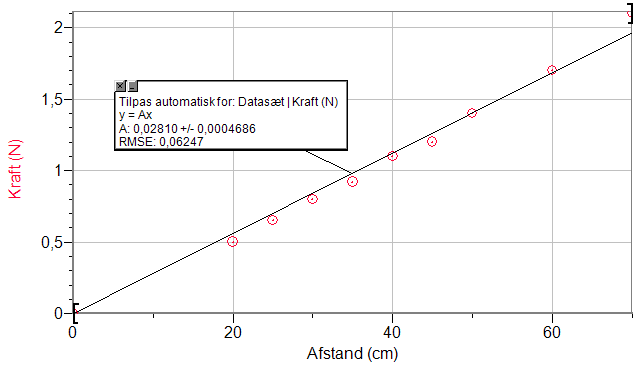
\includegraphics[scale=0.7]{Billeder/graf1}
\end{center}

Vi kan konkludere ud fra $Root-mean-square$-værdien, der er på 0.06247, at en proportionel regression passer godt på den målte data. Altså må Hookes lov $F=k \cdot x$ gælde. Ydermere kan vi sige at fjederkonstanten for den pågældende fjeder har en værdi på $k=0.0281\frac{N}{cm} = 2.81 \frac{N}{m}$
\\

Den data, der ligger til grunde for forsøget kan ses i bilag (MANGLER) 
\\

\subsection{Forsøg 2}
I dette forsøg blev en fjeder, ikke den samme som i forsøg 1, monteret til et stativ og et lod blev hængt i fjederen. Med en Go!Motion ultralydssensor blev afstanden til loddet målt til en sammenhørende tid. Ultralydssensoren var sat til en computer og sendte automatisk data ind i programmet LoggerPro der behandlede dataen og plottede den. Der blev foretaget en regression på datapunkterne på formen $x = A \cdot (B \cdot t + C) + D$. Dette kan ses på følgende billede: 
\begin{center}
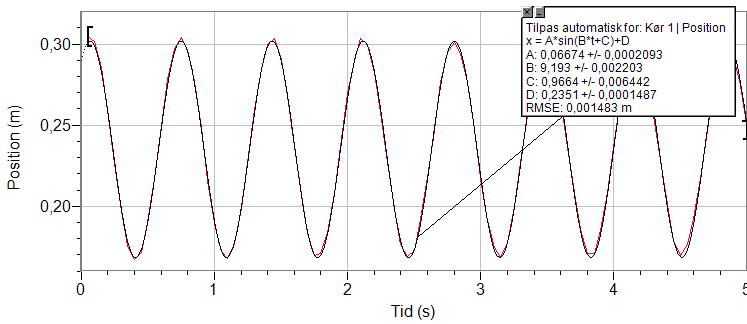
\includegraphics[scale=0.7]{Billeder/graf2}
\end{center}

Som det fremgår af $root-mean-square$-værdien af den regression der er lavet over dataen passer den definerede funktion fantastisk. Det var dette vi gerne ville vise. Herved har vi vist at en oscillerende bevægelse kan skrives på formen: $x = A \cdot (B \cdot t + C) + D$, hvor $B=\sqrt[2]{\dfrac{k}{m}}$. Vi definerer nogle gange $\omega = \sqrt[2]{\dfrac{k}{m}}$ så forskriften kommer til at blive $x(t) = A \cdot (\omega t + C) + D$.

\subsection{Forsøg 3}
I dette forsøg blev 2 fjedre, identiske til den som blev brugt i forsøg 1, hængt op på et stativ og et lod blev sat til dem og loddet blev sat i bevægelse. En Go!Motion ultralydssensor målte afstanden til loddet til en tid og plottede det i programmet LoggerPro. Plottet så sådan ud:

\begin{center}
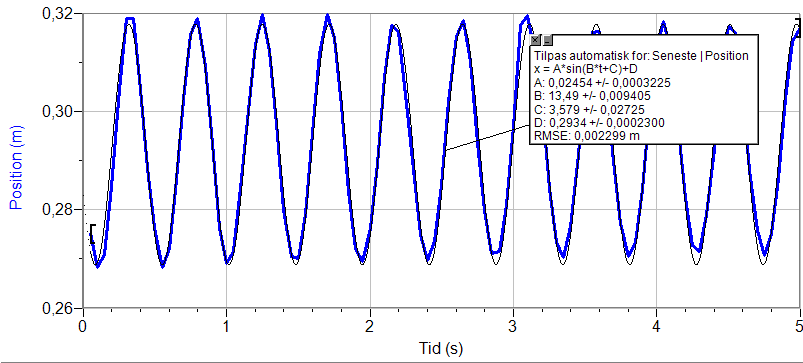
\includegraphics[scale=0.7]{Billeder/graf3}
\end{center}

Her kan vi se, at værdien for B eller $B = \omega = \sqrt[2]{\dfrac{k}{m}}=13.49$. Men da vi kender massen af loddet som blev brugt som $m=32.45g$ (Denne værdi blev målt inden forsøget) Kan vi beregne fjederkonstanten af dette system som:
$k=\omega^2 \cdot m = \frac{13.49}{s} \cdot 32.45g = 5.879 \frac{N}{m}$. Men da vi fandt ud af at fjederkonstanten for forsøg 1 var $k=2.81\frac{N}{m}$ skulle den forventede fjederkonstant for dette forsøg være $2 \cdot 2.81 \frac{N}{m}= 5.62 \frac{N}{m}$. Det målte viste sig at være $5.879 \frac{N}{m}$, hvilket er meget tæt på den forventede værdi. Vi konkluderer da at et system bestående af 2 af de samme fjedre får en fjederkonstant der er lig summen af de 2 fjedre der er med i systemet. 

\subsection{Forsøg 4}
I dette forsøg skulle der undersøges fjederkonstanten for en dobbeltbinding, som består af 2 $\pi-bindinger$ og en enkelt $\sigma-binding$. I forsøget blev der derfor brugt 3 fjedre, hvor 2 af fjedrene var ens. Fjedrene blev hængt op på et stativ og en lodbåd med en vægt i blev sat sammen med fjedrene. De enkelte fjederkonstanter for fjedrene var hhv. $k_1 = 2.74 \frac{N}{m} $ og $17.03 \frac{N}{m}$. Der var 2 fjedre med fjederkonstanten $k_1$ og vi forventede da at fjederkonstanten for systemet blev $k_{system}= 2 \cdot k_1 + k_2$. Lodbåden med vægten i blev sat i bevægelse og en Go!Motion ultralydssensor sendte data til computeren, der i programmet LoggerPro behandlede dataen og plottede følgende:

\begin{center}
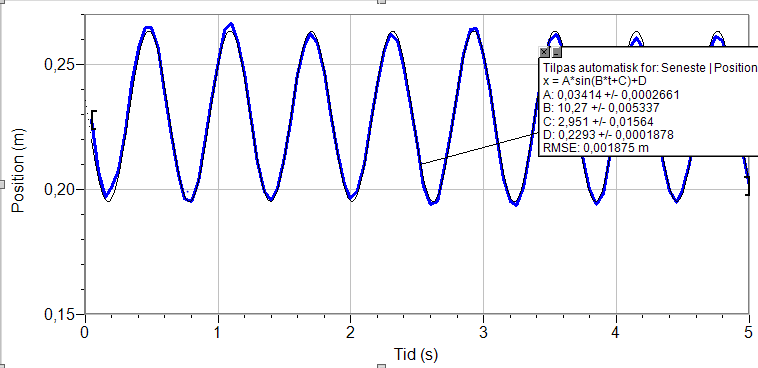
\includegraphics[scale=0.7]{Billeder/graf4}
\end{center}
\section{Den bagvedlæggende kemi}
Stort set alle kemiske forbindelser, der indeholder kovalente bindinger absorberer nogle specielle frekvenser af elektromagnetisk stråling i den infrarøde del af det elektromagnetiske spektrum.\refSpektroskopi{13} Det interval vi beskæftiger os med når vi ser på IR-spektroskopi ligger i intervallet $2,5 \mu m- 25 \mu m $. Det er de bølgelængder af det infrarøde lys, som giver den vibrationelle effekt på atomerne og molekylerne som vi søger. Når vi i afsnit \ref{IRSPEK} skal se på 3 forskellige IR-spektre, vil der hen af x-aksen være plottet reciprokke centimeter. Dette skyldes, at kemikere af konvention laver bølgelængder om til \textbf{bølgetal}, \={v} , ved at tage den reciprokke værdi af bølgelængden i cm.\refSpektroskopi{13}

\begin{center}
\={v}$= \dfrac{1}{\lambda}$
\end{center}

Den primære grund til at bølgetal foretrækkes over bølgelængde er, at bølgetallene er direkte proportionelle til energien af de fotoner, som lyset består af. På den måde vil et højere bølgetal repræsenterer en højere energi. Bølgetal kan laves om til en frekvens ved at gange det med lysets hastighed, c, for så at puttes ind i formlen for fotonenergi $E_{fot} = h \cdot f$, hvor h er plancks konstant og f er frekvens i $\frac{1}{s}$. 
\\

Det ses at fotonenergien bliver større ved et større bølgetal 
\\

\begin{center}
$f =$ \={v} $\cdot c \rightarrow$ \={v} $\cdot c \cdot h = E_{fot}$
\end{center}

Som med alle former for stråling vil molekyler der rammes blive exciteret til et højere energiniveau ved absorbtion af den infrarøde stråling. Det resultat der gør IR-spektroskopi interessant er, at  forskellige molekyler svinger med forskellige frekvenser og derfor optager forskellige bølgelængder af lys. De frekvenser som molekylerne absorberer svarer lige præcist til de egenfrekvenser som molekylerne får når atomerne, der er bundet sammen af kovalente bindinger, enten bøjer eller svinger som vist på figur \ref{fig:spek}. 
\\

Siden alle bånd har en forskellig egenfrekvenser, da de befinder sig i lidt forskellige $miljøer$, vil to molekyler give forskellige udslag på et infrarødt spektrum.\refSpektroskopi{15} Selvom nogle absorbtionsmønstre kan være de samme - hvis begge molekyler eksempelvis indeholder en fælles funktionel gruppe - vil de to molekyler stadigvæk give nogle udslag som adskiller sig fra hinanden, medmindre at stofferne selvfølgelig er identiske. IR-spektre for kemiske forbindelser kan på den måde betragtes den kemiske pendant til menneskets fingeraftryk. Dette betyder at bindinger mellem atomer vil give udslag i små intervaller, der er kendetegnende for netop disse bindinger. Eksempelvis vil et udslag i området $2150cm^{-1}$ formegentligt være 2 carbonatomer, der er tribbeltbundet til hinanden og 2 carbonatomer der er dobbeltbundet til hinanden vil blive fundet området omkring $1650cm^{-1}$. Vi kan slå disse værdier op i en databog
\\

Atomerne i molekylerne der er bundet sammen af kovalente bånd kan svinge på forskellige måder. De simpleste vibrationelle bevægelser i molekyler, som er $infrarøde$ $aktive$ er bindinger som strækker sig eller bøjer.
\\

Der er andre, mere komplicerede måder, som bindingerne mellem atomerne i molekylerne kan opføre sig på. De kan også $sakse$ (scissoring), $rokke$ (rocking), $twiste$ (twisting) og $rykke$ (wagging). 
\\

\begin{center}
\begin{figure}
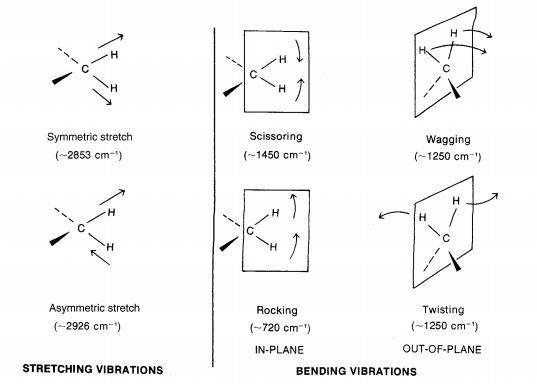
\includegraphics[scale=1]{Billeder/streak}
\caption{Illustration af forskellige vibrationer: Billedet er fra s. 16 i "Introduction to Spectroscopy" \label{fig:spek}}
\end{figure}
\end{center}

Lad os nu se på hvordan vi kan beregne bølgetal for bestemte atom- og funktionelle grupper. Hvis vi nu ser på et af de simpleste eksempler for vibrationer mellem atomer; et diatomisk molekyle med en strækkende vibration. Her kan vi betragte den kovalente binding mellem de to atomer som en fjeder. Et diatomisk molekyle kan betragtes som en fjeder hvor båndlængden bliver ved med at ændre sig. Dette betyder nødvendigvis at den kovalente binding, eller fjederen, må have en frekvens som den vibrerer med. Det gælder at energien for en harmonisk oscillerende bevægelse mellem atomer er direkte proportionelt med frekvensen for den harmoniske oscillator givet ved formlen

\begin{center}
\begin{equation}
E_{osc} \propto h f_{osc}
\end{equation}
\end{center}

For et diatomisk molekyle er det, der bestemmer frekvensen i den harmonisk oscillerende bevægelse størrelserne, k (fjederkonstanten) og masserne af de to atomer der indgår i bindingen $m_1$ og $m_2$.
\\

Frekvensen for en harmonisk oscillerende vibration mellem to atomer er givet ved formlen:

\begin{center}
\={v}$= \dfrac{1}{2 \pi c} \sqrt[2]{\dfrac{k}{\mu}}$
\end{center}

Denne formel er udledt fra Hookes lov for vibrerende fjedre.\refSpektroskopi{18} her er k, fjederkonstanten, \={v} er bølgetallet og $\mu$ er den reducerede masse givet ved formlen $\mu = \frac{m_1 m_2}{m_1 + m_2}$. 
\\

Da det ikke altid er lige praktisk at bruge massen af atomer til at finde bølgetallet, kan man i stedet omskrive lidt på formlen således at der kan regnes på molarmassen af de to atomer i stedet for deres masse.
\\

I stedet for $\mu = \dfrac{m_1 m_2}{m_1 + m_2}$ kan vi skrive $\mu = \dfrac{m_1 m_2}{m_1 + m_2} = \dfrac{M_1 M_2}{(M_1 + M_2 ) (6.02 \cdot 10^{23})}$. 
\\

Vi kan altså udtrykket masserne som molarmasser ved at dividere $\mu$ udtrykt ved masse, med Avogadros tal $N_A$.
\\

Avogadros tal flyttes ud foran kvadratrodstegnet ved at tage kvadratroden af det og putte det i tælleren på den første brøk således at der står:

\begin{center}
\={v}$(cm^{-1})=\dfrac{\sqrt[2]{6.02 \cdot 10^{23}}}{2 \pi c} \cdot \sqrt[2]{\dfrac{K}{\mu}} = \dfrac{7.76 \cdot 10^{11}}{2 \pi c} \cdot \sqrt[2]{\dfrac{K}{\mu}}$
\end{center}

Her er $\mu$ ikke massen længere, men \emph{molarmassen}.
\\

Udtrykket kan reduceres yderligere ved at udregne værdien af den  første brøk, så vi får formlen

\begin{center}
\={v}$=4.12 \sqrt[2]{\dfrac{K}{\mu}}$
\end{center}

Hvor $\mu$ er den reduerede molarmasse og k er fjederkonstanten for systemet i \emph{dynes} per. centimeter. Dynes er mål for kraft. $10^5$  $dynes = 1N$.
\\

Som en approksimation bruger vi respektivt K = 5, 10, 15 $\cdot 10^5 \frac{dynes}{cm}$ for enkelt, dobbelt og trippeltbindinger.
\\

For at validere denne formel vil vi se på 2 eksempler hvor bølgetallet er bestemt gennem et eksperiment sammenligne det med de værdier der opnås når formlen bruges. Vi betragter først dobbeltbindingen mellem carbonatomerne i ethen.
\\

Det bølgetal, der er bestemt ved forsøg er \={v}$=1650cm^{-1}$\refSpektroskopi{21}. Hvis vi bruger formlen til at regne bølgetallet ud får vi: $4.12 \cdot \sqrt[2]{\dfrac{10 \cdot 10^5}{(\frac{12 \cdot 12}{12 +12})}} = 1682 cm^{-1}$. 
\\

Et andet eksempel er bindingen mellem et carbonatom og et hydrogenatom. Her er der tale om en enkeltbinding og vi bruger da $K=5 \cdot 10^5 \frac{dynes}{cm}$ og en $\mu = \frac{12 \cdot 1}{12 + 1} = 0.9231$. Putter vi det ind i formlen får vi et bølgetal på: $4.12 \cdot \sqrt[2]{\dfrac{5 \cdot 10^5}{0.9231}} \approx 3032 cm^{-1}$. Bølgetallet for stræk mellem C og H er ved forsøg bestemt til at være 3000.\refSpektroskopi{21} 
\\

Formlen giver os altså et godt bud på hvor vi kan forvente at se bølgetal for stræk mellem to atomer.
\\

Vi vil lige diskutere betydningen af k samt hvad der har indflydelse på størrelsen af k. 
\subsection{Fjederkonstanten for bindingen mellem diatomiske molekyler}

I normale fjedre vil fjederkonstanten, som navnet antyder, være konstant lige gyldigt hvad vi hænger i den. Dette gør sig egentligt også gældende for de kovalente bindinger mellem molekyler, hvis de vel at mærke er underlagt præcist de samme betingelser. 
\\

Et større k medfører et større bølgetal, da tælleren bliver større og værdien for $\sqrt[2]{\dfrac{K}{\mu}}$ da bliver større. Det er derfor vigtigt, at se på de faktorer der bestemmer værdien af k.
\\

\textbf{Betydninger for værdien af k}
\begin{enumerate}
\item Det gælder som en regel at værdien af fjederkonstanten, k, er tre gange så høj for tripeltbindinger som for enkeltbindinger og at k er dobbelt så høj for dobbeltbindinger som for enkeltbindinger. Vi sætter disse værdier af k til at være henholdsvis 5, 10 og 15 for enkelt-, dobbelt- og trippeltbindinger. Vi vil senere diskutere i hvor stor grad denne tommelfingerregel for beregninger af bølgetal holder.

\item Hybdridisering har også en effekt på værdien af k. Som regel er bånd stærkere i rækkefølgen $sp > sp^2 > sp^3$. Dette kan vi se hvis vi betragter enkeltbundne, dobbeltbundne og trippeltbundne carbonatomer, der også binder sig til et hydrogenatom:

\begin{center}
\begin{figure}
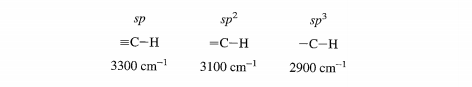
\includegraphics[scale=1]{Billeder/sp}
\caption{Billedet er fra s. 19 i "Introduction to Spectroscopy"}
\end{figure}
\end{center}


\end{enumerate}

For det andet vil store atomer der er bundet til atomer, der er relativt mindre end dem selv vibrerer ved højere frekvenser, da værdien af $\mu$ vil være mindre og gøre $\sqrt[2]{\dfrac{K}{\mu}}$ større. 
\\

Vi kan tjekke om dette passer ved at slå op i en databog og se på bølgetal for forskellige atomer bundet sammen:
\\
\begin{figure}
\includegraphics[scale=1]{Billeder/udklip}
\caption{Billedet er taget fra s. 18 i "Introduction to Spectroscopy"}
\end{figure}

Billedet viser, at jo større et atom carbon er bundet til jo større bliver $\mu$ og derfor også bølgetallet \={v}.

Bevægelser mellem atomer, der er bøjende vil også optræde ved en lavere energi, og altså også ved et lavere \={v}, end de strækkende bevægelser. Eksempelvis vil C-H stræk give udslag ved et bølgetal på ca. 3000 $cm^{-1}$ mens C-H bøj vil give et udsalg omkring $1340cm^{-1}$.

\subsubsection{Hookes lov som model for interaktion mellem atomer}
I forrige afsnit fandt vi frem til formlen:

\begin{center}
\={v}$=4.12 \sqrt[2]{\dfrac{K}{\mu}}$
\end{center}

Denne formel utrolig brugbar til at regne bølgetal ud for vibrationer mellem to atomer. Vi skal dog notere os, at formlen kun kan bruges til at regne bølgetallet ud for strækkende vibrationer mellem to atomer, da formlen er udledt ud fra Hookes lov, som beskriver en fjeder som bliver enten trukket i eller presset sammen. Formlen beskriver altså ikke de andre former for \emph{vibrationer} som buk, saks og tvist.
\\

Derudover bruger vi i den selv samme formel følgende værdier for k: $5 \cdot 10^5 dynes$ for enkeltbindinger, $10 \cdot 10^5 dynes$ for dobbeltbindinger og $15 \cdot 10^5 dynes$ for trippeltbindinger. Vi viste, at disse værdier passede godt for de to eksempler med methan og ethen, men hvis vi husker hvad vi fandt ud af i \ref{sec:del} ville fjederkonstanten for et system være lig summen af alle de fjederkonstanter, som var med i systemet.
\\

Antag at fjeder-/kraftkonstanterne for henholdsvis enkelt-, dobbelt- og tripeltbininger er $5 \cdot, 10 \cdot$ og $15 \cdot 10^5 dynes$. Der vil nu føres et argument for at disse værdier af k leder til en absurditet. 
\\
\textbf{Da enhederne i følgende argument er de samme undlades de i regnestykket af simplicitet}
\\
Hvis vi ser på et system med en dobbeltbinding skal fjeder-/kraftkonstanten være 10. Da en dobbeltbinding også indeholder en $\sigma$-binding kan vi tillade os jævnførende resultatet i \ref{sec:del} at trække fjederkonstanten for en $\sigma$-binding fra, som er 5. Dette efterlader os med en fjederkonstant på 5 som vi skal tildele til de resterende fjedre i systemet. Da vi kun har en $\pi$-binding tilbage må vi enten have at $\pi$-bindingen er lige så stærk som $\sigma$-bindingen, hvilket er falskt. Eller, hvis vi regner $\pi$-bindingen som 2 svage fjedre over for hinanden på hver sin side af $\sigma$-bindingen, at $\sigma$-bindinger er præcist dobbelt så stærke som $\pi$-bindinger - hvilket også er falskt.
\\

Derfor er antagelsen om at enkelt-, dobbelt- og trippeltbindinger respektivt kan gives værdierne $5 \cdot, 10 \cdot$ og $15 \cdot 10^5 dynes$ for k en antagelse og ikke et udtryk for værdiens virkelighed. 
\section{IR-analyse af stofferne paracetamol, ibuprofen og R-limonen}
Vi vil i dette afsnit se nærmere på hvordan man i praksis bestemmer hvilket stof et bestemt IR-spektrogram hører til. Der vil ses på de tre stoffer: paracetamol, som er et udbredt smertestillende middel, ibuprofen, der også er smertestillende og til sidst stoffet R-limonen, som er en farveløs væske der ved stuetemperatur dufter kraftigt af appelsin (FODNOTE WIKI). Vi har tre forskellige stoffer vi skal tildele til tre forskellige IR-spektre. Man kan indledningsvist se på molekylernes opbygning og gøre det klart for sig selv, hvilke steder man forventer at se absorption. 
\\

Der kigges da på de funktionelle grupper som de tre stoffer indeholder

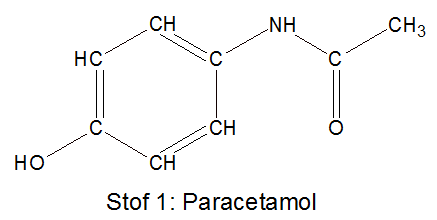
\includegraphics[scale=0.5]{Billeder/paracetamol}
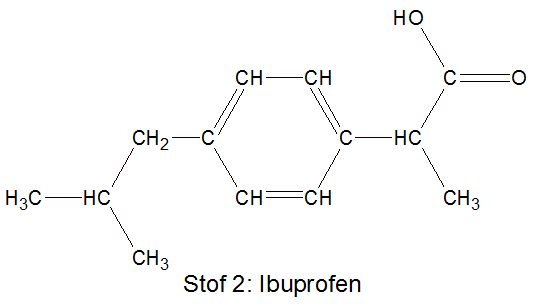
\includegraphics[scale=0.5]{Billeder/ibuprofen}
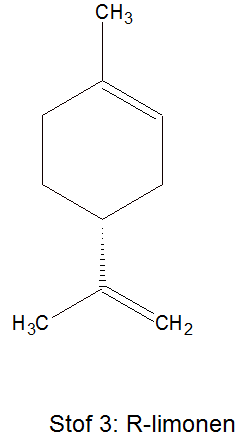
\includegraphics[scale=0.5]{Billeder/Rlimonen}
\begin{enumerate}
\item[\textbf{Stof 1}] 
Stof 1 er paracetamol. De karakteristiske bølgetal for funktionelle grupper vi har tænkt at at kigge efter, når vi skal slå op i vores tabel for bølgetal er følgende: 
\begin{enumerate}
\item Fenol, da vi har en alkoholgruppe, som sidder på en aromatisk ring. 

\item hj
\end{enumerate}

Fenol, da vi har en alkoholgruppe, som sidder på en aromatisk ring. 
\item[\textbf{Stof 2}]

\item[\textbf{Stof 3}]

\end{enumerate}
\section{Konklusion}
Med udgangspunkt i de forsøg som blev foretaget og behandlet i denne opgave står det nu klart, at Hookes lov gør sig gældende for \emph{perfekte} fjedre. Derudover har det også vist sig at positionen for objekter bundet til fjedre, der sættes i bevægelse foretager harmonisk oscillerende bevægelser, som kan beskrives ud fra en funktion på formen: $x(t)=A \cdot (\omega t + C) + D$. Af dette resultat kunne frekvensen for en harmonisk oscillerende bevægelse bestemmes som: $f=\frac{1}{2\pi} \cdot \sqrt[2]{\frac{k}{m}}$, der i afsnittet om bestemmelse af bølgetal relaterede sig direkte til bestemmelsen af bølgetallet \={v}. Teorien om de karakteristiske egenfrekvenser for funktionelle grupper gjorde det muligt gennem en analyse af de funktionelle grupper i paracetamol, ibuprofen og R-limonen at kunne knytte de tre stoffer til hvert deres IR-spekrum.
\section{Litteraturliste}
\subsection*{Litteratur}
Mygind, Helge; Nielsen, Ole Vesterlund; Axelsen Vibeke: "BASISKEMI C": Århus: Haase og søns forlag: 2010
\\

Holtzclaw, Henry F.; Robinson, William R.; Nebergall, William H: "General Chemistry": USA: D. C. Heath and Company: 1984
\\

Ole Vesterlund; Axelsen Vibeke: "BASISKEMI A": Århus: Haase og søns forlag: 2011
\\

Alberty, Robert A.: "Physical chemistry": Singapore: John Wiley and sons: 1987
\\

Sears, Francis W.; Zemansky, Mark W.; Young, Hugh D.: "University Physics": USA: Addison-Wesley: 1987
\\

Pavia, Donald L.; Lampman, Gary M.; Kriz, George S.: "Introduction to spectroscopy": USA: Thomson Learning: 2001

\subsection{Hjemmesider}
https://da.wikipedia.org/wiki/Limonen Besøgt (20-12-2016 kl. 23:05)

\end{document}